\chapter{Homological algebra}\label{chapter:hom_alg}

References for this chapter are \cite{weibel, hom_algebra}.

\section{Chain complexes}

	\newdef{Chain complex}{\index{chain!complex}\index{boundary}\index{differential}\index{cycle}\label{homalg:chain_complex}
		\nomenclature[S_CH]{$C_\bullet$}{Chain complex}
		\nomenclature[S_CHCat]{$\textbf{Ch}_bullet(\textbf{A})$}{Category of chain complexes with objects in the additive category $\textbf{A}$.}
		Let $\mathbf{C}$ be an additive category (often an Abelian category). Consider a sequence $(A_k)_{k\in\mathbb{Z}}$ of objects and a sequence $\{\partial_k:A_k\rightarrow A_{k-1}\}_{k\in\mathbb{Z}}$ of morphisms in $\mathbf{C}$ (called the \textbf{boundary operators} or \textbf{differentials}) such that for all $k\in\mathbb{Z}$:
		\begin{gather}
			\partial_k\circ\partial_{k+1} = 0
		\end{gather}
		This structure is called a chain complex\footnote{A \textbf{cochain complex} is constructed similarly. For this structure we consider an ascending order, i.e. $\partial_k:A_k\rightarrow A_{k+1}$.}. Elements of $\text{im}(\partial_k)$ are called \textbf{boundaries} and elements of $\text{ker}(\partial_k)$ are called \textbf{cycles}. The chain complex $\{(A_k, \partial_k)\}_{k\in\mathbb{Z}}$ is often denoted by $(A_\bullet, \partial_\bullet)$ or simply by $A_\bullet$ if the choice of boundary operators is clear.
	}

	The morphisms of chain complexes are called \textbf{chain maps} and they are defined as a collection of morphisms $\{f_k:A_k\rightarrow B_k\}_{k\in\mathbb{Z}}$ such that for all $k\in\mathbb{Z}$ the following equation holds:
	\begin{gather}
		\partial'_k\circ f_k = f_{k-1}\circ\partial_k
	\end{gather}
	where $\partial_k, \partial_k'$ are the boundary operators of respectively $A_\bullet$ and $B_\bullet$. Given an additive category $\mathbf{C}$ one can define the category $\mathbf{Ch}_\bullet(\mathbf{C})$ of chain complexes and chain maps in $\mathbf{C}$, this category is often denoted by $\mathbf{Ch}_\bullet(\mathbf{C})$.

	\remark{Given a chain (resp. cochain) complex $C$ one can easily construct a cochain (resp. chain) complex $\tilde{C}$ by setting $\tilde{C}_k = C_{-k}$.}

	\newdef{Chain homology}{\index{homology}\label{homalg:homology}
		Given a chain complex $C_\bullet$ one can define its homology groups $H_n(C_\bullet)$. Since $\partial^2=0$ the kernel $\ker(\partial_k)$ is a subgroup of the image $\im(\partial_{k+1})$. This way we can define the quotient groups:
		\begin{gather}
			H_n(C_\bullet) := \frac{\ker(\partial_k)}{\im(\partial_{k+1})}
		\end{gather}
		The kernel in this definition is often called the group of \textbf{cycles} and is denoted by $Z_k(C_\bullet)$. The image in this definition is often called the group of \textbf{boundaries} and is denoted by $B_k(C_\bullet)$.
	}

	\newdef{Quasi-isomorphism}{
		Consider a chain map $f_\bullet:C_\bullet\rightarrow D_\bullet$. If the induced maps on homology are isomorphisms then $f_\bullet$ is called a quasi-isomorphism.
	}

	\newdef{Chain homotopy}{\index{chain!homotopy}
		Two chain maps $f_\bullet, g_\bullet: C_\bullet\rightarrow D_\bullet$ are said to be chain homotopic if there exists a chain map $s_\bullet:C_\bullet\rightarrow D_\bullet$ such that the following equation is satisfied:
		\begin{gather}
			f-g = s\circ\partial_C + \partial_D\circ s
		\end{gather}
		If both $f\circ g$ and $g\circ f$ are chain homotopic to the identity then $C_\bullet$ and $D_\bullet$ are said to be (chain) homotopy equivalent.
	}

	\begin{property}
		Every (chain) homotopy equivalence is a quasi-isomorphism.
	\end{property}

\section{Exact sequences}

	\newdef{Exact sequence}{\index{exact!sequence}
		Let $\mathbf{C}$ be an additive category (often an Abelian category). Consider a sequence (finite or infinite) of objects and morphisms in $\mathbf{C}$:
		\begin{gather}
			A_0\xrightarrow{\Phi_1}A_1\xrightarrow{\Phi_2}\cdots\xrightarrow{\Phi_n}A_n
		\end{gather}
		This sequence is said to be exact if for every $k\in\mathbb{N}: \text{im}(\Phi_k) = \text{ker}(\Phi_{k+1})$. In particular this means that $\Phi_{k+1}\circ\Phi_k = 0$ for all $h\in\mathbb{N}$ and as such this implies that exact sequences are a special type of chain complex as defined in definition \ref{homalg:chain_complex}.
	}

	\newdef{Short exact sequence}{
		A short exact sequence is an exact sequence of the form:
		\begin{gather}
			\label{short_exact_sequence}
			0\rightarrow A_0\xrightarrow{\Phi_1}A_1\xrightarrow{\Phi_2} A_3\rightarrow0
		\end{gather}
		A long exact sequence is an infinite exact sequence.
	}

	\begin{property}
		\index{epimorphism}\index{monomorphism}\index{bimorphism}
		Looking at some small examples we can derive some important constraints for certain exact sequences and especially for short exact sequences. Consider the sequence
		\[
			0\rightarrow A\xrightarrow{\Phi} B
		\]
		This sequence can only be exact if $\Phi$ is an injective homomorphism (\textbf{monomorphism}). This follows from the fact that the only element in the image of the map $0\rightarrow A$ is 0 because the map is a homomorphism. The kernel of $\Phi$ is thus trivial which implies that $\Phi$ is injective.

		Analogously, the sequence
		\[
			A\xrightarrow{\Psi}B\rightarrow0
		\]
		is exact if $\Psi$ is a surjective homomorphism (\textbf{epimorphism}). This follows from the fact that the kernel of the map $B\rightarrow0$ and thus the image of $\Psi$ is all of $B$ which implies that $\Psi$ is surjective.

		It follows that the sequence
		\[
			0\rightarrow A\xrightarrow{\Sigma}B\rightarrow0
		\]
		is exact if $\Sigma$ is a \textbf{bimorphism} (which is often an isomorphism).
	\end{property}

\section{Resolutions}

	Consider some Abelian category $\textbf{A}$. Let $\textbf{Ch}(\textbf{A})$ denote the category of chain complexes with objects in $\textbf{A}$. In fact in this and coming sections we will only be interested in chain complex concentrated in positive degree, i.e. $C_k=0$ for all $k<0$, and henceforth we will assume that all chain complexes satisfy this condition.

	\newdef{Acyclic complex}{
		A chain complex $C_\bullet\in\mathbf{Ch}(\mathbf{A})$ is said to be acyclic if the sequence \[\cdots\longrightarrow C_{k+1}\longrightarrow C_k\longrightarrow C_{k-1}\longrightarrow\cdots\]
		is exact.
	}
	\sremark{
		Some references, especially the older ones, use a slightly different definition of acyclicity. In their definition the sequence is exact except in degree 0, i.e. $H_0(C_\bullet)\neq0$.
	}

	\newdef{Resolution}{\index{augmentation!map}
		Consider an object $X\in\ob{A}$. A resolution of $X$ is given by a chain complex $C_\bullet\in\mathbf{Ch}(\mathbf{A})$ which is acyclic except in degree 0 with the property that $H_0(C_\bullet)\cong X$. This definition is equivalent to stating that there exists an exact sequence of the form
		\begin{gather}
			\cdots\longrightarrow C_1\longrightarrow C_0\overset{\varepsilon}{\longrightarrow} X\longrightarrow 0
		\end{gather}
		The morphism $\varepsilon:C_0\rightarrow X$ is often called the \textbf{augmentation map}.
	}

	Often one can or should specialize the type of resolution. For example by considering chain complexes with only injective or projective objects (see figures \ref{fig:injective_object} and \ref{fig:projective_object}), one obtains injective or projective resolutions.

	If every object $X\in\ob{A}$ admits a projective (resp. injective) resolution then $\mathbf{A}$ is said to have enough projectives (resp. injectives).

\section{Derived functors}

	Given an additive functor (see definition \ref{category:additive_functor}) one can define its \textbf{prolongation} on the category of chain complexes:
	\newdef{Prolongation}{
		Let $\func{F}{A}{A'}$ be an additive functor. Consider the categories of chain complexes $\textbf{Ch}(\mathbf{A})$ and $\textbf{Ch}(\mathbf{A'})$. The prolongation of $F$ is a functor $\overline{F}:\textbf{Ch}(\textbf{A})\rightarrow\textbf{Ch}(\textbf{A}')$ obtained by applying $F$ to every object in a chain complex and to every diagram in the definition of a chain map.
	}

	To understand and unify the various long exact sequences in (co)homology and to give general statements about these theories we introduce the concept of derived functors.

	\newdef{Left derived functor}{\index{functor!derived}
		Let $\mathbf{A}$ be an Abelian category with enough projectives and consider a right exact functor $\func{F}{A}{A'}$. The left derived functors $L_iF$ are defined in the following way. Pick an object $X\in\ob{A}$ and construct a projecive resolution $P_\bullet\xrightarrow{\varepsilon}X\rightarrow0$. Apply the prolongation $\overline{F}$ to this resolution and construct its chain homology $H_\bullet$. The left derived functors are then given by:
		\begin{gather}
			L_iF(X) := H_i(\overline{F}P_\bullet)
		\end{gather}
		Right derived functors (in the case of a left exact functor $F$) can be constructed dually by choosing an injective resolution, applying the prolongation and taking the cohomology of the resulting cochain complex. In the remainder of this section we will always work with left derived functor for simplicity.
	}

	\remark{The above construction is valid for covariant functors. For contravariant functors one has to change it slightly. For contravariant functors $F$ one calculates the derived functors of the opposite functor $F^{op}$. This is equivalent to starting with an injective (resp. projective) resolution for the calculation of left (resp. right) derived functors since injective objects are projective in the opposite category and similarly homology becomes cohomology in the opposite category.}

	\begin{property}
		If $F$ is exact the above construction immediately implies that the derived functors vanish identically.
	\end{property}

	\begin{property}\label{hom:projective_object}
		Consider a right exact functor $F$ together with its left derived functors $L_iF$. If an object $P$ is projective then $L_iF(X)=0$ for all $i\geq1$. This can easily be proven by remarking that every projective object $P$ admits a projective resolution of the form \[\cdots\longrightarrow0\longrightarrow0\longrightarrow P\longrightarrow P\longrightarrow0\]
	\end{property}

	Now of course we could wonder why the resolutions used in the construction of derived functors are required to be projective or injective. This seems to be a very strong requirement. The reason for this is that using our definition one obtains naturally isomorphic derived functors, i.e. the result is independent of the resolution used.

	However for some cases one would like to work with a more general resolution. For example in the next section, when considering the tensor product it would be great to just work with \textit{flat} modules. To this intent we introduce the following notion:
	\newdef{Acyclic resolution}{\index{acyclic!object}
		Consider a right exact functor $F$ together with its left derived functors $L_iF$. An object $X$ is said to be \textbf{$F$-acyclic} if $L_iF(X)=0$ for all $i\geq 1$. A resolution of an object $Y$ is said to be ($F$-)acyclic if all objects in the resolution are $F$-acyclic.

		It can be proven that calculating the derived functors of $F$ with respect to an $F$-acyclic resolution gives functors isomorphic to the ones obtained using the construction introduced above.
	}

	One of the motivating applications of derived functors is the relation with the exactness of a functor and the relation to various long exact sequences in (co)homology theories. All of these are a result of the following property:
	\begin{property}
		Let $\func{F}{A}{A'}$ be a right exact (additive) functor (the left exact case proceeds in a similar way). Consider a short exact sequence in $\mathbf{A}$:
		\begin{gather}
			0\longrightarrow A\longrightarrow B\longrightarrow C\longrightarrow 0
		\end{gather}
		Now choose projective resolutions for $A$ and $C$. By the \textit{horseshoe lemma} we obtain a projective resolution for $B$ which fits in a short (split) exact sequence of chain complexes:
		\begin{gather}
			0\longrightarrow A_\bullet\longrightarrow B_\bullet\longrightarrow C_\bullet\longrightarrow 0
		\end{gather}
		Since $F$ is additive and the above sequence is split exact the induced complex is also split exact, i.e. the following sequence is exact
		\begin{gather}
			0\longrightarrow\overline{F}A_\bullet\longrightarrow\overline{F}B_\bullet\longrightarrow\overline{F}C_\bullet\longrightarrow0
		\end{gather}
		is exact and so the \textit{zig-zag lemma} is applicable. This theorem gives us the following long exact sequence in homology:
		\begin{gather}
			\cdots\longrightarrow H_i(\overline{F}B_\bullet)\longrightarrow H_i(\overline{F}C_\bullet) \longrightarrow H_{i-1}(\overline{F}A_\bullet) \longrightarrow H_{i-1}(\overline{F}B_\bullet) \longrightarrow\cdots
		\end{gather}
		These homology groups are by definition the same as the left derived functors ($L_i = H_i\circ\overline{F}$) and accordingly we have a long exact sequence relating the different derived functors.
	\end{property}
	\begin{result}
		By the above long exact sequence of derived functors we see that the first derived functor gives the obstruction to $F$ being an exact functor. Since exact functors have vanishing derived functors we obtain the following result:
		\begin{gather}
			L_1F = 0\implies L_iF=0\ \ \forall i\geq 1
		\end{gather}
	\end{result}

\subsection{Module categories}\label{section:tor_ext}

	Let us first consider the tensor and hom bifunctors $-\otimes-$ and Hom$(-, -)$. The tensor functor is right exact in both arguments while the hom functor is left exact in both arguments and hence we can form the associated left and right derived functors. For simplicity we will always work in the first argument. A proof that the derived functors are \textit{balanced}, i.e. that one can use a projective resolution for either argument and obtain isomorphic results, can be found in the references cited in the beginning of the chapter.

	\newdef{Tor-functor}{\index{Tor}
		Consider a finite group $G$ and a $G$-module $B$. The Tor-functors Tor$^n_G(-, B)$ are defined as the left derived functors of the tensor functor $-\otimes_{\mathbb{Z}G} B$.
	}

	\newdef{Ext-functor}{\index{Ext}
		Consider a finite group $G$ and a $G$-module $A$. The Ext-functors Ext$_n^G(-, A)$ are defined as the right derived functors of the hom functor Hom$_{\mathbb{Z}G}(-, A)$.
	}

	For module categories over a ring one can use a simpler technique. For every module $M$ one can construct a free resolution: Choose a free module which maps $F_0$ onto $M$; then choose a free module $F_1$ which maps onto the kernel of the map $p_0:F_0\rightarrow M$ and so forth. So without further ado we will always assume the resolutions to be free.

\subsection{Group cohomology}\index{cohomology!finite groups}\label{section:group_cohomology}

	In this section we will give an application of derived functors. In differen areas of mathematics and physics the concept of group cohomology pops up, e.g. group extensions, projective representations and symmetry-protected topological order. These applications however often start from an a priori ad hoc construction based on maps from a group $G$ to a $G$-module (we will come back to this point further below).

	For simplicity we will only consider finite groups and Abelian coefficients groups. Every (Abelian) $G$-module can be regarded as a module over the group ring $\mathbb{Z}[G]$, i.e. there exists an equivalences of categories between $\mathbf{Ab}$ and $\mathbb{Z}[G]$-$\mathbf{Mod}$. Assuming the axiom of choice, every module category over a ring has enough projectives and hence it makes sense to define group (co)homology\footnote{In fact most types of (co)homology for rings, algebras and modules can be defined this way.} using derived functors. For groups we will give an explicit construction of a resolution which is not just $\mathbb{Z}[G]$-projective but even $\mathbb{Z}[G]$-free.

	The homology and cohomology of a finite group $G$ with coefficients in a $G$-module $A$ is defined using the Ext- and Tor-functors defined above:
	\begin{align}
		H^\bullet(G; A) &:= \text{Ext}_{\mathbb{Z}[G]}^\bullet(\mathbb{Z}, A)\\
		H_\bullet(G; A) &:= \text{Tor}^{\mathbb{Z}[G]}_\bullet(A, \mathbb{Z})
	\end{align}
	where $\mathbb{Z}$ carries the trivial $G$-module structure. To explicitly calculate the (co)homology groups we have to find a $\mathbb{Z}[G]$-projective resolution of $\mathbb{Z}$:
	\begin{construct}[Normalized bar resolution]\index{resolution!bar}
		Let $P'_n$ be the free $\mathbb{Z}[G]$-module on $G^n$. The boundary maps are defined as follows:
		\begin{gather}
			\label{hom_group_boundary}
			\partial_k(g_1, ..., g_k) = g_1(g_2, ..., g_k) + \sum_{i=1}^k (-1)^i(g_1, ..., g_ig_{i+1}, ..., g_k) + (-1)^k (g_1, ..., g_{k-1})
		\end{gather}
		To obtain the normalized bar\footnote{One of the possible explanations for this name is that the formal generating elements are often written as $[g_1|g_2|...|g_k]$.} resolution (in inhomogeneous form) one has to quotient out the submodule of $P'_n$ generated by tuples $(g_1,..., g_n)$ where one of the $g_i$'s is the identity. It can be shown that the resulting quotient modules $P_n$ form a $\mathbb{Z}[G]$-free (in particular $\mathbb{Z}[G]$-projective) resolution of $\mathbb{Z}$.
	\end{construct}

	To explicitly calculate the cohomology groups $H^k(G; A) = H^k(\text{Hom}_{\mathbb{Z}[G]}(P_\bullet, A))$ it is often easier to work with a more explicit description of the involved Hom-sets. Since $P'_k$ is the free $\mathbb{Z}[G]$-module on $G^k$, it is isomorphic (as a module) to $\mathbb{Z}[G^{k+1}]$. This can be seen as follows. The generating set consists of all $k$-tuples of elements in $G$: \[S = \{(g_1, ..., g_k): g_i\in G, \forall i\leq k\}\] Since we generate a module over $\mathbb{Z}[G]$, we can write every element as formal combination over $\mathbb{Z}$ of elements of the form \[g_0(g_1, ..., g_k)\] where the multiplication, regarded as the (left) $G$-action, between $g_0$ and the $k$-tuple is merely formal. We can now construct a morphism $\varphi$ between this module and $\mathbb{Z}[G^{k+1}]$, which carries the diagonal $G$-action, in the following way. On the generating set $S$ we define $\varphi$ to be:
	\begin{gather}
		\varphi(g_1, ..., g_k) = (e, g_1, g_1g_2, ..., g_1g_2\cdots g_k)
	\end{gather}
	It is not hard to show that morphism is in fact an isomorphism (of $G$-modules) and hence we find that
	\begin{gather}
		H^k(G; A) = H^k(\text{Hom}_{\mathbb{Z}[G]}(\mathbb{Z}[G^{k+1}], A))
	\end{gather}
	By a little more algebra it can also be shown that this Hom-set is isomorphic to the (set-theoretic) mapping space Map$(G^k, A)$. This space can be given an Abelian group structure induced by the group structure of $A$. Combining these facts we get the following construction for the cohomology of groups:
	\begin{construct}[Group cohomology]
		Let $G$ be a finite group and let $A$ be a $G$-module. Let $C^k$ be the free Abelian group generated by the set-theoretic functions $f:G^k\rightarrow A$ with the property that if any of its arguments is the identity then the result is 0. The boundary maps $\partial^k$, induced by the maps defined in equation \ref{hom_group_boundary}, are given by:
		\begin{gather}
			(\partial^k f)(g_1, ..., g_{k+1}) = g_1\cdot f(g_2, ..., g_{k+1}) + \sum_{i=1}^k(-1)^if(..., g_ig_{i+1}, ...) + (-1)^{k+1}f(g_1, ..., g_k)
		\end{gather}
		This is exactly the relation used to obtain group cohomology in definition \ref{group:cohomology}.
	\end{construct}

	\begin{property}[Finiteness]
		Let $G$ be a finite group and let $A$ be a $G$-module such that the underlying group is finitely generated. Since in this case the Hom-groups are finitely generated, the cohomology groups $H^k(G; A)$ with $k\geq1$ are also finitely generated. Furthermore, they are annihilated by the order of $G$ so in particular they are all torsion. It follows that all cohomology groups are finite.
	\end{property}

\section{Spectral sequences}

	\sremark{In this section we will adopt the homological convention, i.e. differentials lower the degree.}

	\newdef{Spectral sequence}{\index{spectral!sequence}\index{page}
		Consider a sequence of differential objects $\{(E_i, d_i)\}$. This sequence is called a spectral sequence if it satisfies
		\begin{gather}
			H(E_i, d_i) = E_{i+1}
		\end{gather}
		for every $i$. A morphism of spectral sequences is a collection of morphism $\{\varphi_i\}$ satisfying:
		\begin{itemize}
			\item $\varphi_i\circ d_i = d_i'\circ\varphi_i$
			\item $\varphi_{i+1} = H(\varphi_i)$
		\end{itemize}
		The objects $E_i$ are often called the \textbf{pages} of the spectral sequence.
	}

\subsection{Exact couples}

	\newdef{Exact couple}{\index{exact!couple}
		An exact ''couple'' is a tuple $(A, B, \alpha, \beta, \gamma)$ such that diagram \ref{fig:exact_couple} commutes.
		\begin{figure}[!ht]
			\centering
			\begin{subfigure}{0.40\textwidth}
				\centering
				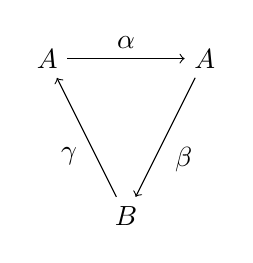
\begin{tikzpicture}
					\node (A) at (-1, 1) {$A$};
					\node (A2) at (1, 1) {$A$};
					\node (B) at (0, -1) {$B$};
					\draw[->] (A) -- node[above]{$\alpha$} (A2);
					\draw[->] (A2) -- node[below right]{$\beta$} (B);
					\draw[->] (B) -- node[below left]{$\gamma$} (A);
				\end{tikzpicture}
				\caption{Exact couple.}
				\label{fig:exact_couple}
			\end{subfigure}
			\begin{subfigure}{0.49\textwidth}
				\centering
				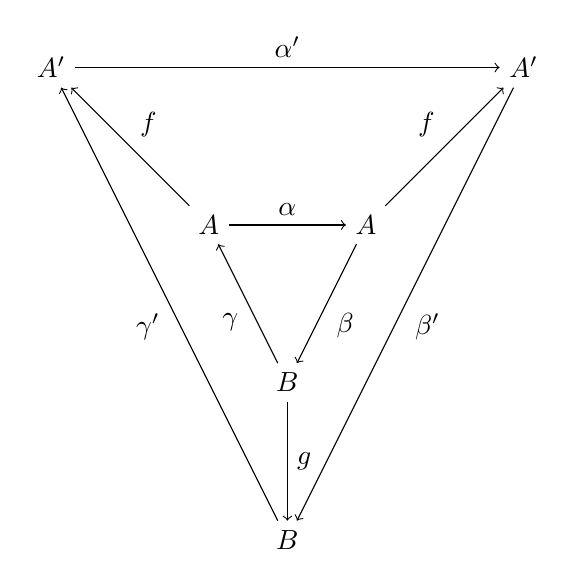
\begin{tikzpicture}
					\node (A') at (-3, 3) {$A'$};
					\node (A2') at (3, 3) {$A'$};
					\node (B) at (0, -1) {$B$};
					\node (A) at (-1, 1) {$A$};
					\node (A2) at (1, 1) {$A$};
					\node (B') at (0, -3) {$B$};
					\draw[->] (A') -- node[above]{$\alpha'$} (A2');
					\draw[->] (A2') -- node[below right]{$\beta'$} (B');
					\draw[->] (B') -- node[below left]{$\gamma'$} (A');
					\draw[->] (A) -- node[above]{$\alpha$} (A2);
					\draw[->] (A2) -- node[below right]{$\beta$} (B);
					\draw[->] (B) -- node[below left]{$\gamma$} (A);
					\draw[->] (A) -- node[above right]{$f$} (A');
					\draw[->] (A2) -- node[above left]{$f$} (A2');
					\draw[->] (B) -- node[right]{$g$} (B');
				\end{tikzpicture}
				\caption{Morphism of exact couples.}
				\label{fig:exact_couple_morphism}
			\end{subfigure}
			\caption{}
			\label{fig:exact_couples_category}
		\end{figure}

		A morphism of exact couples is a pair of morphisms $(f, g):(A, B)\rightarrow (A', B')$ that make the diagram \ref{fig:exact_couple_morphism} commute.
	}

	From any exact couple $(A, B, \alpha, \beta, \gamma)$ one can construct a spectral sequence using the following prescription:
	\begin{align}
		E_0 &= B\\
		d_0 &= \beta\circ\gamma\\
		&\nonumber\\
		E_n &= \frac{\gamma^{-1}(\alpha^n(A))}{\beta(\alpha^{-n}(0))}\\
		d_n &= \beta\circ\alpha^{-n}\circ\gamma
	\end{align}
	It is not so hard to see that $E_{n+1}=H(E_n, d_n)$, so this construction gives a functor from the category of exact couples to the category of spectral sequences. The higher exact couples $(\alpha^nD, E_n, \dots)$ are sometimes called \textbf{derived couples}.

	One can also define the term $E_\infty$ using the following limit procedure: For every $n$ one can look at the elements in $E_n$ that are closed under $d_n$, let's call them $E_{n,n+1}$. Since there exists a canonical surjection $E_{n,n+1}\rightarrow E_{n+1}$ one can then look at all the elements in $E_{n,n+1}$ for which their image in $E_{n+1}$ is closed under $d_{n+1}$ and call these $E_{n,n+2}$. The elements that remain after taking the limit of this operation form the set $E_{n, \infty}$. Now we can also take the (direct) limit of these $E_{n,\infty}$ and this gives us $E_\infty$. This is equivalent to
	\begin{gather}
		E_\infty = \frac{\cap_i Z(E_i)}{\cup_i B(E_i)}
	\end{gather}
	Hence $E_\infty$ contains the equivalence classes of elements that are cycles for all $d_n$ but boundaries for none. If $E_\infty$ is the associated graded object of some filtered object $G$ then we say that the spectral sequence \textbf{converges} to $G$.

	Now consider a differential object $(C, d)$ together with a filtration\footnote{See definition \ref{set:filtration}.} $\{F_pC\}_{p\in\mathbb{N}}$. The definition of the filtration immediately gives us a short exact sequence for every $p\in\mathbb{N}$:
	\begin{gather}
		0\longrightarrow F_{p-1}C\longrightarrow F_pC\longrightarrow F_pC/F_{p-1}C\longrightarrow0
	\end{gather}
	This short sequence then gives rise to a long exact sequence in homology, which can be expressed as an exact triangle, and this triangle in turn leads to an exact couple:
	\begin{gather}
		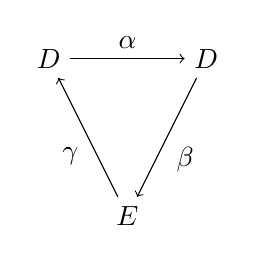
\begin{tikzpicture}
			\node (A) at (-1, 1) {$D$};
			\node (A2) at (1, 1) {$D$};
			\node (B) at (0, -1) {$E$};
			\draw[->] (A) -- node[above]{$\alpha$} (A2);
			\draw[->] (A2) -- node[below right]{$\beta$} (B);
			\draw[->] (B) -- node[below left]{$\gamma$} (A);
		\end{tikzpicture}
	\end{gather}
	where $D_p = H(F_pC)$ and $E_p=H(F_pC/F_{p-1}C)$. From a more abstract (but at the same time more useful) point of view one can consider the object $E$ as a functor from the category of filtered (differential) objects to the category of graded objects. As such it is constructed from the composition of the homology functor $H$ and the \textit{associated graded object-functor} \[Gr:C\rightarrow \{G_pC := F_pC/F_{p-1}C\}_{p\in\mathbb{N}}.\]

	On the other hand we could of course also construct the composition $Gr\circ H$ which first maps a differential object to its homology object and then builds the graded object associated to the filtration \[F_pH(C):=\im\left(H(F_pC)\rightarrow H(C)\right).\] Now of course some interesting questions arise: ''\textit{How are the functors $H\circ Gr$ and $Gr\circ H$ related?}'', ''\textit{Do they coincide?}'', ... The latter question is easy to answer, namely ''\textit{No, they do not.}'' However they can be related and this happens through a spectral sequence that will tell us how the homology of the graded object associated to $C$ can be related to the homology of $C$ itself.

\subsection{Filtered complexes}

	For the remainder of this section we will only consider graded differential objects, i.e. $C_\bullet=\{C_p\}_{p\in\mathbb{Z}}$ for which $dC_p\subseteq C_p$. In this case the exact couple now consist of $D=\{D^{p,q}:=H_q(F_pC_\bullet)\}$ and $E=\{E_{p,q}:=H_q(G_pC_\bullet)\}$ and hence the objects are now bigraded. (The filtration is also required to preserve the differential, i.e. $dF_iC_j\subseteq F_iC_{j-1}$.)

	\sremark{In contrast to most of the literature we did not adopt the \textit{complementary convention}, i.e. the convention where $p+q$ denotes the total degree and hence $E_{p,q}=H_{p+q}(G_pC_\bullet)$.}

	Before we introduce an expression for a general page $E_r$ we will consider the degree zero and one terms to get some intuition. The differential on $E_0$ is given by
	\begin{gather}
		d_0:\frac{F_pC_q}{F_{p-1}C_q}\rightarrow\frac{F_pC_{q-1}}{F_{p-1}C_{q-1}}
	\end{gather}
	and is induced by the differential $d$ on $C_\bullet$. The kernel of this map is clearly given by all elements $x\in F_pC_q$ such that $dx = 0\mod F_{p-1}C_{q-1}$ (with the additional remark that we also have to take the quotient by $F_{p-1}C_q$). As a result we find that the homology $E_1=H(E_0, d_0)$ is given by
	\begin{gather}
		E_1^{p,q}:=\frac{\{x\in F_pC_q: dx\in F_{p-1}C_{q-1}\}}{F_{p-1}C_q+dF_pC_{q+1}}.
	\end{gather}
	The first term in the denominator was already explained above. The second term comes from the $\im(d_0)$ part in the definition of $H(E_0, d_0)$. One might suspect that some data is missing since the relevant map $d_0^{p, q+1}$ goes from $\frac{F_pC_{q+1}}{F_{p-1}C_{q+1}}$ to $\frac{F_pC_q}{F_{p-1}C_{q}}$. However, the image of $F_{p-1}C_{q+1}$ is a subspace of $F_{p-1}C_q$ and this is already included in the first term, so we might as well work with all of $F_pC_{q+1}$.

	For arbitrary $r>0$ we define the page $E_r$ as follows:
	\begin{gather}
	E_r^{p,q}:=\frac{\{x\in F_pC_q: dx\in F_{p-r}C_{q-1}\}}{F_{p-1}C_q+dF_{p+r-1}C_{q+1}}.
	\end{gather}